\documentclass[11pt]{article}
\usepackage[dvips]{graphicx, color}
\usepackage{epsfig}
\usepackage{amsmath}
\usepackage{mathptmx}

\setlength{\evensidemargin}{-0.7cm}
\setlength{\oddsidemargin}{-0.0cm}
\setlength{\textwidth}{15.5cm}
\setlength{\topmargin}{-2cm}
\setlength{\textheight}{23.5cm}
\parskip 1ex    % White space between paragraphs amount
\parindent 0pt

\usepackage{html}
\usepackage[ruled]{algorithm2e}
%\usepackage{varioref}
%\usepackage[breaklinks=true,pagebackref=true]{hyperref}
%\hypersetup{colorlinks=true,urlcolor=black,citecolor=blue}

\newcommand{\red}{\color{red}}
\newcommand{\green}{\color{green}}
\newcommand{\blue}{\color{blue}}

\graphicspath{{Figures/}}

\begin{document}

\title{MSTransform Framework in CASA}
\author{Sandra Castro and Justo Gonzalez}
\date{07 February 2013, (last modified : 16 December 2014)}
\maketitle

This memo describes the MSTransform module in CASA as available from version
4.1.0 onwards.
%Section \ref{Sec:CodeDocs} gives an outline of the software implementation. 
Section \ref{Sec:Running} 
describes what 
various transformations do, with some examples and suggestions on how to use them in
Section \ref{Sec:Examples}. 
Section \ref{Sec:FAQ} contains a list of frequently-asked questions and their answers.

This is a living document. Details will continue to be added (with examples). Feedback is welcome.

\tableofcontents

%\section{Software Documentation}

\subsection{C++ Infrastructure}\label{Sec:CodeDocs}

\subsubsection{Framework}
%{\green Link to (or copy of) Justo's documentation of the infrastructure design, 
%with links from each 'class' box/section to the relevant doxygen code-doc pages. }

\paragraph{Main Classes}

\begin{enumerate}
\item
%\htmladdnormallink{AgentFlagger}{http://www.eso.org/~scastro/ALMA/casa/active/CasaRef/agentflagger-Tool.html}:
%\htmladdnormallink{AgentFlagger}{http://casa.nrao.edu/active/docs/CasaRef/agentflagger-Module.html}:
\htmladdnormallink{AgentFlagger}{http://casa.nrao.edu/docs/CasaRef/agentflagger-Module.html}:
The top-level AgentFlagger class that connects all of the following together, and defines the C++ user-interface 
for the agentflagger.  
This is the class used by the tool layer.

%\item \htmladdnormallink{FlagDataHandler}{http://www.eso.org/~jagonzal/Flagging-3.4-Docs/html/classcasa_1_1FlagDataHandler.html} : A top level class defining the data handling interface for the flagging module. 
\item \htmladdnormallink{FlagDataHandler}{http://casa.nrao.edu/docs/doxygen/html/classcasa_1_1FlagDataHandler.html} : 
A top level class defining the data handling interface for the flagging module. 

\item The  \htmladdnormallink{FlagAgentBase}{http://casa.nrao.edu/docs/doxygen/html/classcasa_1_1FlagAgentBase.html} 
base class defines the behaviour of all flagging agents
and contains agent-level data-selection, etc.  The main functions to be implemented by derived classes are
setAgentParameters(), preProcessBuffer(), computeAntennaPairFlags() or computeRowFlags(), getReport() . 

List of available Flag Agents : 
\begin{enumerate}
\item \htmladdnormallink{FlagAgentManual}{http://casa.nrao.edu/docs/doxygen/html/classcasa_1_1FlagAgentManual.html} :  
Flag/Unflag based on data-selections.  
The only processing done by this agent is to set the flags for all data it sees to 
True if the operation is to flag, and to False to unflag. A boolean parameter
apply determines whether to flag (apply=True) or unflag (apply=False). By
default it is set to True.

\item \htmladdnormallink{FlagAgentQuack}{http://casa.nrao.edu/docs/doxygen/html/classcasa_1_1FlagAgentQuack.html} :  
Flag time-ranges at the beginning and/or end of scans. 
Uses the YYY iteration-mode. 

\item \htmladdnormallink{FlagAgentElevation}{http://casa.nrao.edu/docs/doxygen/html/classcasa_1_1FlagAgentElevation.html} : 
Flag time-ranges based on source elevation. 
Uses the YYY iteration-mode.

\item \htmladdnormallink{FlagAgentShadow}{http://casa.nrao.edu/docs/doxygen/html/classcasa_1_1FlagAgentShadow.html} : 
For each timestep, flag antennas that are shadowed by
any other antenna.  Antennas to be flagged are chosen and marked in the preProcess() stage.
Rows are flagged in computeRow(), and this agent uses the YYY iteration-mode.

\item \htmladdnormallink{FlagAgentExtend}{http://casa.nrao.edu/docs/doxygen/html/classcasa_1_1FlagAgentExtension.html} : 
Read and extend flags along specified axes, within the
current chunk.  Uses the YYY iteration-mode.

\item \htmladdnormallink{FlagAgentClip}{http://casa.nrao.edu/docs/doxygen/htmlclasscasa_1_1FlagAgentClipping.html} : 
Flag based on a clip threshold and visExpression.
Find and flag NaNs and Infs.  Uses the YYY iteration-mode. 

\item \htmladdnormallink{FlagAgentTimeFreqCrop}{http://casa.nrao.edu/docs/doxygen/html/classcasa_1_1FlagAgentTimeFreqCrop.html} : 
The TFCrop algorithm is run per
baseline, via FlagAgentTimeFreqCrop::computeAntennaPairFlags()

\item \htmladdnormallink{FlagAgentRFlag}{http://casa.nrao.edu/docs/doxygen/html/classcasa_1_1FlagAgentRFlag.html} : 
The RFlag algorithm. 
Implements multiple passes through each chunk via the  passIntermediate() and passFinal() mechanism.

\item \htmladdnormallink{FlagAgentSummary}{http://casa.nrao.edu/docs/doxygen/html/classcasa_1_1FlagAgentSummary.html} : 
Flag counts are accumulated in computeRow()
and packaged into a Record in getResult(). 

\item \htmladdnormallink{FlagAgentDisplay}{http://casa.nrao.edu/docs/doxygen/html/classcasa_1_1FlagAgentDisplay.html} : 
Visibilities are read and displayed from computeAntennaPair(). Navigation-buttons control the order in which the framework iterates through baselines. 

\end{enumerate}



\item The \htmladdnormallink{FlagReport}{http://casa.nrao.edu/docs/doxygen/html/classcasa_1_1FlagReport.html} class allows each flag agent to build and return 
information (summary counts, reports as plots, etc) to the user (and/or) to the display agent
for end-of-MS reports.
\end{enumerate}


\subsubsection{Control Flow}
%{\green  Justo, if you have a nicer way to describe the control flow, then please replace this part,  but otherwise, just this text-algorithm may be good-enough for this document (after it's completed).  If you already have the different iteration-modes explained somewhere (in one of the .h files), we can just point to it from here.  }


%%% For documentation on how to use this syntax, see the PDF file from here : 
%%  http://www.ctan.org/tex-archive/macros/latex/contrib/algorithm2e/

\begin{algorithm}
  \SetLine
%  \linesnumbered
  \dontprintsemicolon
  \vspace{0.5cm} 
  \KwData{Pre-selected Measurement Set}
  \KwIn{List of Flag Commands}
  \KwOut{Flags updated in-place + summaries/reports}
  \vspace{0.5cm} 
  {Setup FlagDataHandler :} \;
  {Build Agent List }\;
  \While (\tcc*[f]{chunks (array,obs,field,spw)}) { more chunks }
  {
    \While (\tcc*[f]{sub-chunks (ntime)}) { more times }
    {
      \ForAll (\tcc*[f]{agents}) { agents }
      {
        \If {agent touches this data}
        {
          {agent :: pre-Process current buffer}\;
             \If {iterationApproach = XXX}
             {
               \ForAll {baselines}
               {
                  {agent :: computeAntennaPairFlags()}\;
               }
             }
             \If {iterationApproach = YYY}
             {
               \ForAll {rows}
               {
                {agent :: computeRowFlags() }\;
               }
             }
        }
      }
    }
    {fdh :: Flush Flag Cube}\;
  }
  {Gather Reports from all agents} \;
\end{algorithm}





\subsubsection{Performance Optimizations}

%{\green  Explanation of various performance-optimization features  }


There are several performance-optimization choices that can be made. 
Some of these are under the users control, and some have automated heuristics.

\paragraph{List mode}

It helps to combine multiple flag commands into a single run ONLY if most of the
commands require the same data to be read.  

The goal is to read data once, apply multiple flag commands, and write flags once.

\begin{enumerate}
\item  Manual-flag commands read only meta-data.
\item  Shadow, elevation read meta-data + processing to calculate uvw, azel.
\item  Clip reads visibilities.
\item  tfcrop and rflag read visibilities and flags
\item Extend, summary read flags
\end{enumerate}



\paragraph{Data pre-selection}
If only a subset of the Measurement Set is to be traversed for flag-calculation,
it helps to pre-select and iterate through only that section of the MS.  
When multiple flag commands are supplied, with different data-selections, 
this pre-selection is calculated as a loose union of all input selection parameters
(currently a list of all unique spectral-windows and field-ids).

This is done automatically at the task level, and is in the control of the user at the 
tool level (via {\tt af.selectdata()}.

Note that there is a second level of selection per agent (command) that ensures
that each agent (command) sees only its correct subset of the data. 
The above pre-selection is purely for optimization reasons to prevent the infrastructure
from stepping through and rejecting untouched parts of the data (even though the
meta-data reads requires for the checks per chunk are minimal). 

\paragraph{Asynchronous I/O}
Asynchronous I/O is a data-access optimization that applies when iterating through the
dataset in chunks.  It uses multi-threading to pre-read the next chunk of data from disk
while the current chunk is being processed.

The user has the option of enabling asynchronous I/O by setting the following 
variables in the .casarc file. 

\begin{verbatim}
VisibilityIterator.async.enabled: true     # if present and set to false then async i/o will work
VisibilityIterator.async.nBuffers: 2       # the default value is two
VisibilityIterator.async.logFile: stderr   # Send async i/o debug log messages to this file
                                           # if not present or file is invalid then no logging occurs
VisibilityIterator.async.logLevel: 2       # Level of log messages to output (two is good, too); defaults to 1

FlagDataHandler.asyncio: true                # True : enable async-IO for the flagger (clip,tfcrop,rflag)
FlagDataHandler.slurp: true                  # True : enable ??
FlagAgent.background: true                   # True : enable threading mode
\end{verbatim}

Asynchronous I/O helps ONLY when data I/O dominates the total cost. 
For our current list of agents/algorithms, this helps only for agents that read 
visibilities. Therefore asynchronous I/O is activated only if clip or tfcrop or rflag 
are present in the flag-command list.


\paragraph{Agent parallelization}

Parallel execution of flagging agents helps when processing dominates the runtime, but there
are several factors that will affect performance. 
Parallelization by agent is helpful only if there is a list of agents of similar type, and the number of
agents is less than the number of available cores.  Parallelization by data-partitioning (chunks of
baselines, for example) is useful if all agents touch all baselines and do not require communication
across baselines).

Agent-level parallelization is currently disabled, but as part of 
\htmladdnormallink{CAS-3861}{https://bugs.nrao.edu/browse/CAS-3861}, heuristics will be implemented internally, and then documented here.



\paragraph{Interaction between Async IO and Agent parallelization}

Figures \ref{Fig:AsyncDiags} symbolically shows how async-IO and agent parallelization would scale
when IO dominates, vs when processing dominates.

\begin{figure}
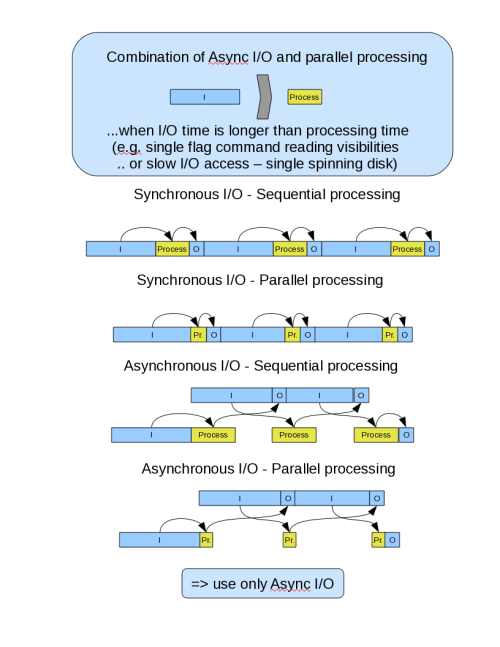
\includegraphics[scale=0.7]{async.parallel.diagram.IOdominates.png}
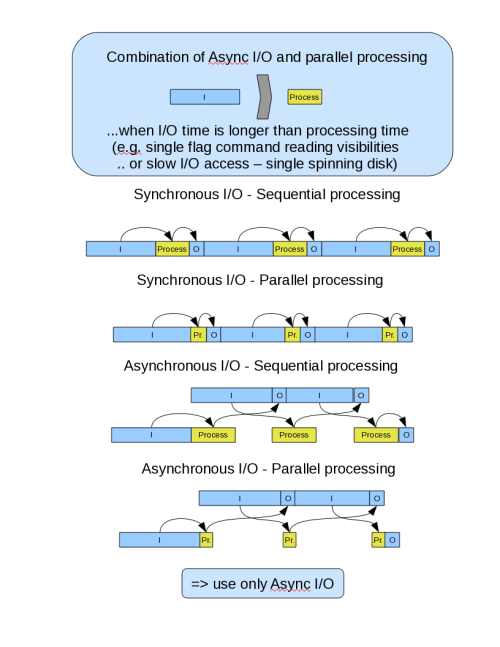
\includegraphics[scale=0.7]{async.parallel.diagram.IOdominates.png}
\caption{Explanation...}
\label{Fig:AsyncDiags}
\end{figure}






\subsubsection{Timing Tests}

Data : 

Continuum : few fat channels.\\
SpectralLine : many thin channels.\\

SinglePointing : contiguous scans on the same field\\
Mosaic  :  each scan is a different fields.\\

\begin{enumerate}
\item \label{dA} L-band continuum , Single Pointing   ----- need to decide dataset (probably G55.7+3.4\_1s.ms)
\item \label{dB} L-band spectral-line , Mosaic            ----- need to pick dataset 

\end{enumerate}


\paragraph{Comparison between modes}
%{\green Tables from Justo for 50 and 150 GB continuum datasets. }


\begin{figure}
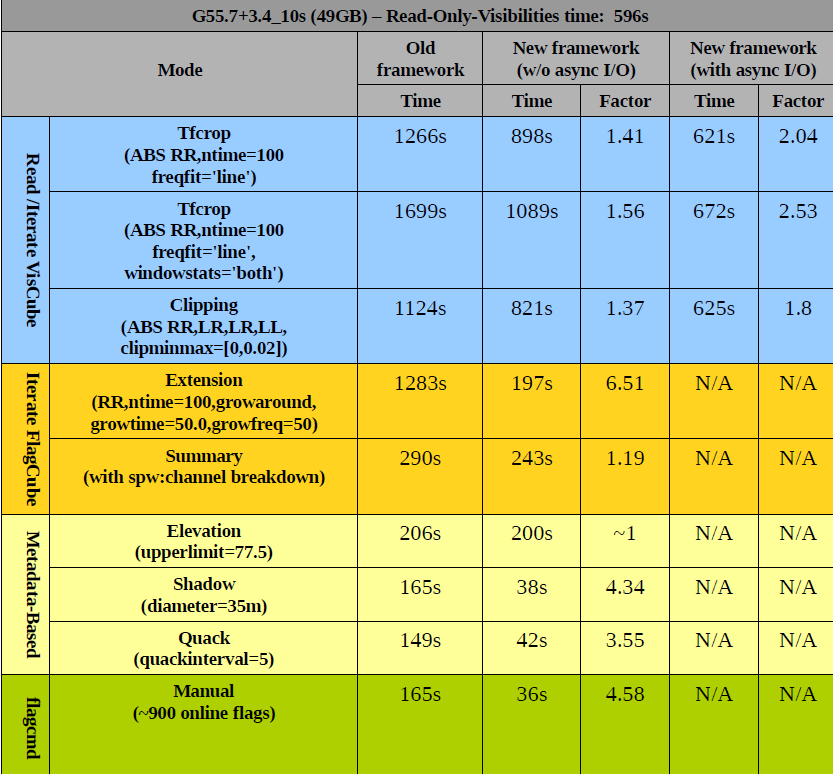
\includegraphics[scale=0.7]{table.timings.50GB.G55data.png}
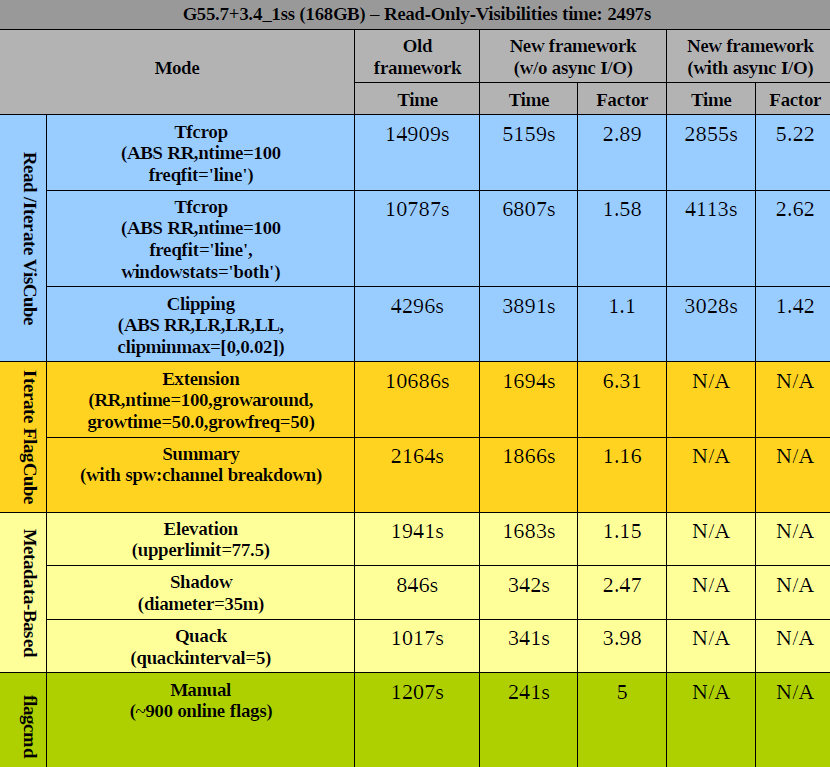
\includegraphics[scale=0.7]{table.timings.150GB.G55data.png}
\caption{These tables show timing comparisons between various modes, for two EVLA continuum datasets. Parameters of the datasets are... }
\end{figure}


\paragraph{Break-down of timings} : if possible, with and without async-IO.
\begin{enumerate}
\item  Only-reading-visibilities 
\item  Only-reading flags
\item  Only-writing flags
\item  (pls ignore if this makes no sense.) Only-iterating through the visbuffers without reading/writing anything (i.e. to see if much time is saved by the loose union). 
\end{enumerate}

\paragraph{Comparison between data-shapes and iteration patterns}

Two types of datasets : wideband continuum single-pointing,   spectral-line mosaic



%%%%%%%%%%%%%%%%%%%%%%%%%%%%%%%%%%%%%%%%%%%%%%%%%%%%
%%%%%%%%%%%%%%         SECTION           %%%%%%%%%%%%%%%%%%%%%%%%%%%
%%%%%%%%%%%%%%%%%%%%%%%%%%%%%%%%%%%%%%%%%%%%%%%%%%%%



\subsection{Python tool and task}\label{Sec:TaskTool}

\subsubsection{agentflagger tool}
\paragraph{Examples how to use the the new flagging framework from the tool.}
All the functions available in the tool are explained
\htmladdnormallink{here.}{http://www.eso.org/~scastro/ALMA/casa/active/CasaRef/agentflagger-Module.html}

\begin{enumerate}
\item Open the MS or a calibration file and attach it to the tool.

The function
takes three arguments, the MS or CAL table, the iteration approach to use and the time interval. 
Only the MS is mandatory to use. By default it will use the
FlagDataHandler::SUB\_INTEGRATION iteration approach and 0.0 seconds as the
time interval.

\begin{verbatim}
    af.open('my.ms')
\end{verbatim}

\item Select the data where to flag. If left blank, the whole MS will be
selected.

This step will use the MS Selection class. There are two functions to perform the
selection. One takes a Python dictionary (Record in C++) of the parameters, the
other takes the individual parameters as arguments.

\begin{verbatim}
  1) First method:
    selection={}
    selection['spw']="0:1~10"
    selection=['scan']="1"
    af.selectdata(selection)

  2) Second method:
    af.selectdata(spw="0:1~10", scan="1")
\end{verbatim}

\item Parse the parameters of the flagging agents.

Now it is time to build a list of the agents that we want to run to process the data. This
step will create a list of all the agents that will be executed to flag/unflag the data.
This method can be called multiple times. Every call should contain the desired parameters of
the agent and optionally data selection parameters. When data selection parameters are present,
the agent will only loop through that portion of the data.

This method will check if the requested agent (mode) is known from the following list
(manual, clip, quack, shadow, elevation, tfcrop, rflag, extend, unflag and summary). If
empty or unknown, it will give a warning and return.

If any tfcrop, rflag or extend mode is present, this method will calculate the maximum value
of time interval (ntime) from these agents. The maximum value will be used for
all the agents in the list.

A similar situation will happen with the combinescans parameter. If any of the combinescans is
True, it will be taken as True to all agents.

Async I/O will be activated if any of the modes clip, tfcrop or rflag is requested.

Only for the tfcrop agent, if a correlation ALL is requested, this method will create one
agent for each available polarization in the MS. For example, if the MS contains polarizations
XX and YY and the parameter is correlation="ABS\_ALL", then there will be two
tfcrop agents, one with correlation="ABS\_XX" and the other with
correlation="ABS\_YY". The apply parameter is set by default to True to apply
the flags.

\begin{verbatim}
     agent_pars = {}
     agent_pars["mode"] = "clip"
     agent_pars["clipzeros"] = true
     agent_pars["apply"] = true
     af.parseagentparameters(agent_pars)

     agent_pars = {}
     agent_pars["mode"] = "manual"
     agent_pars["autocorr"] = true
     af.parseagentparameters(agent_pars)

     agent_pars = {}
     agent_pars["mode"] = "summary"
     agent_pars["basecnt"] = true
     af.parseagentparameters(agent_pars)
\end{verbatim}

There are convenience functions to parse the agent's parameters, one specific for each agent.
The above calls can be done instead using these functions.

\begin{verbatim}
     af.parseclipparameters(clipzeros=true, apply=true)
     af.parsemanualparameters(autocorr=true)
     af.parsesummaryparameters(basecnt=true)
\end{verbatim}

In either one of the cases, three agents will be created. We need to initialize the agents, which
will call the constructor of each one of them and set the parameters that were given in the previous
calls. Some basic checks will be performed at this stage for types and values of the parameters.

If any tfcrop, rflag, extend or display agent is in the list, the iteration approach will be
set to a different value depending on whether combinescans is true or not. When True, the
iteration approach will be set to
FlagDataHandler::COMBINE\_SCANS\_MAP\_ANTENNA\_PAIRS\_ONLY, otherwise to
FlagDataHandler::COMPLETE\_SCAN\_MAP\_ANTENNA\_PAIRS\_ONLY.

\item Initialize the agents.

This method will create agents and add them to a FlagAgentList. If for any reason, the call to
FlagAgentBase::create(fdh\_p, agent\_rec) fails, an error message will be
displayed. Any agents previously added to the FlagAgentList will remain there. A subsequent call to this method can be done to add
more agents to the same FlagAgentList.

\begin{verbatim}
     af.init()
\end{verbatim}

\item Process the flags and write them to the MS.

The run method takes two parameters, writeflags and sequential.
The parameter writeflags controls whether to write the flags or not to the MS.
By default it is set to True. Setting writeflags to False is useful when one
wants to run the tool together with the display agent to see what is going to be
flagged before deciding to write or not to the MS. The sequential parameter
controls if the order of the agent's list is to be preserved or not. If set to
False, the order will not be preserved and the framework may execute the agent's list in parallel.
By default sequential is set to True.

The run method gathers several reports, depending on wich agents are run. The display and summary agents
produce reports that can be retrieved from calling the run method. The reports are returned via a Python
dictionary. When executed from the task, only the report of the
last summary in the list will be returned. If executed from the tool level,
multiple reports are allowed for the summary agent.

In the previous example, only one summary agent was added to the list, therefore
two reports will be returned in the dictionary. The first report contains the
summaries per field, spw, scan, correlation, etc. The second report
gives the antenna positions for plotting.

\begin{verbatim}
     my_reports = af.run()
\end{verbatim}

\item Destroy the tool.

\begin{verbatim}
    af.done()
\end{verbatim}
 \end{enumerate}
 
\paragraph{The following are only possible in the tool.}
\begin{enumerate}

\item Run multiple summary agents in a list. In order to do this, add as many
summary agents are desired when parsing the agent's parameters. You can do this by
calling the af.parseagentparameters() several times before calling af.init().

\item Determine to run the agents in sequential or in parallel. Set the
'sequential' parameter of the run method to True or False to control this.

\end{enumerate}

\paragraph{Explain the heuristics applied for the automatic activation of async
I/O and parallel run}

\subsubsection{flaghelper functions}

This Python file contains many helper functions for flagdata and flacmd. The
functions can be imported inside casapy.

\begin{verbatim}
     import flaghelper as fh
\end{verbatim}

\subsubsection{flagdata task}
Help for the flagdata task is available \htmladdnormallink{here.}
{http://casa.nrao.edu/docs/taskref/flagdata-task.html}

\subsubsection{flagcmd task}
Help for the flagcmd task is available \htmladdnormallink{here.}
{http://casa.nrao.edu/docs/taskref/flagcmd-task.html}



%%%%%%%%%%%%%%%%%%%%%%%%%%%%%%%%%%%%%%%%%%%%%%%%%%%%





\section{The MSTransform framework}\label{Sec:Running}
% Add parts from Justo's document.
% I/O improvement by avoiding read/write to disk multiple times.
% order of running the transformations
% independence of each transformation.
% new VI???
The mstransform task has been designed to be a single place for many
common operations used in the pre-imaging steps of interferometric
data reduction. It does almost everything done by hanningsmooth,
partition, split and cvel, and more. The task has the following capabilities,
which can be done independently or combined. Except for split which is the default 
state of the task, each transformation has a boolean parameter to switch it on
or off.

\begin{enumerate}
\item Split into a new MS using data selection parameters.
\item Partition into a new Multi-MS using data selection parameters.
\item Combination of spectral windows.
\item Channel averaging using channelized FLAG and WEIGHT/SIGMA\_SPECTRUM (if
present) as the weights.
\item Hanning smoothing.
\item Reference frame transformation, similar to cvel.
\item Separation of spectral windows, which does not have an independent
boolean switch, but it can be independently applied when regridms=True and
the nspw parameter is set to > 1.
\item Time averaging using channelized FLAG and WEIGHT/SIGMA\_SPECTRUM (if
present) as the weights.

\end{enumerate}

Mapping of parameters between split-mstransform and cvel-mstransform.

\begin{verbatim}

    split               mstransform                                      Comments
 -----------------------------------------------------------------------------------------------------
    width               chanaverage=True, chanbin                        perform channel averaging
    timebin             timeaverage=True, timebin                        perform time averaging
    combine             timeaverage=True, timespan                       time averaging with time spanning
    keepflags           keepflags                                        keep or drop flags in output


\end{verbatim}


\begin{verbatim}


    cvel                mstransform                                      Comments
 -----------------------------------------------------------------------------------------------------
    hanning             hanning=True                                     Hanning smoothing
    other parameters    combinespws=True, regridms=True, cvel parameter  regrid the MS
    ---                 regridms=True, nspw                              does not exist in cvel

\end{verbatim}


Documentation for the task and tool can be found in:
\htmladdnormallink{Task Documentation}{http://casa.nrao.edu/docs/TaskRef/TaskRef.html}
\htmladdnormallink{Tool Documentation} {http://casa.nrao.edu/docs/CasaRef/CasaRef.html}

\subsection{Splitting capabilities}
Task mstransform behaves like split in all cases that concern sub-table re-indexing
and selection. It does not support multiple channel selections (separated by a
semi-colon) within one spw. If there is an spw selection, it will re-index the
spws starting from 0.

The mstransform task is able to work with MSs that contain spectral windows with 
different polarization shapes. Split cannot handle such MSs, but this was overcome 
in mstransform.

A data column specifies which column will be used for the transformations. It is
possible to make real a virtual MODEL column, by setting the parameter
{\it datacolumn} to any of the values 'model', 'all' or 'data,model,corrected'
and then setting the sub-parameter {\it realmodelcol} to True. This will copy the virtual
column to a physical MODEL column in the MS main table. The virtual model column
will be deleted afterwards.

The user can control whether to create WEIGHT\_SPECTRUM/SIGMA\_SPECTRUM columns
in the output MS or not. If the input MS does not have a
WEIGHT\_SPECTRUM/SIGMA\_SPECTRUM column, by setting the parameter {\it
usewtspectrum} to True, the task will create a WEIGHT\_SPECTRUM from the values
in the WEIGHT column, and initialize SIGMA\_SPECTRUM to 1/sqrt(WEIGHT\_SPECTRUM). 
By default, {\it usewtspectrum} is set to False.

The resulting WEIGHT\_SPECTRUM produced by mstransform is in the statistical
sense correct for the simple cases of channel average and time average, but not for the 
general re-gridding case, in which the error propagation formulas applicable for 
WEIGHT\_SPECTRUM are yet to be defined. Currently, as in cvel and in the imager,
WEIGHT\_SPECTRUM is transformed in the same way as the other data columns,
notice that this is not formally correct from the statistical point of view, but is a good
approximation at this stage.

The parameter {\it keepflags} from split is also available in mstransform. By
default, mstransform keeps the flagged data in the output, depending on the data
selection parameters. Regardless of this parameter, flagged data is never used
in channel averaging. When {\it keepflags} is set to False, only partially
flagged rows will be used in time averaging. This behavior is different from
split.

\begin{verbatim}
    mstransform('uid.ms', outputvis='myout.ms', datacolumn='data', spw='0:21~120,3,5')
  will select 100 channels from spw 0 and all of spw 3 and 5
\end{verbatim}

\subsection{Multi-MS Structure}
A Multi-MS (MMS) is structured to have a reference MS on the top directory and a subdirectory
called SUBMSS, which contains each partitioned sub-MS. A Multi-MS can be
handled like a normal monolithic MS. It can be moved and renamed like any other
directory. CASA tasks that are not MMS-aware can process it like a monolithic MS.
The reference MS contains links to the sub-tables of the first sub-MS. The other sub-MSs
contain a copy of the sub-tables each. In order to reduce the volume of the MMS, the
POINTING and SYSCAL tables (which are read-only in all use cases and identical for all
sub-MSs) are stored only with the first sub-MS and linked into the other sub-MSs.

The table.info file inside the reference MS contains information on the axis used to partition
the original MS. This information is written by the partition task and carried over by other
tasks.

\subsection{Partition and Multi-MS support}
The partition task is the main task to create a Multi-MS. It takes an input Measurement Set
and creates an output Multi-MS based on the data selection parameters. Partition accepts three
axis to do separation across: auto, scan or spw. The default auto will first separate the MS in
spws, then in scans. Each partitioned MS is referred to as a sub-MS. The user
may force the number of sub-MSs in the output MMS by setting the parameter {\it numsubms}.
By default, the parameter {\it createmms} is set to True to create an output
MMS.

If set to False, the task will work as the split task and create a normal MS based on the input data selection.
Task partition uses two helper classes to handle the parallel jobs; ParallelTaskHelper and
ParallelDataHelper. Special care needs to be
taken in order to consolidate the sub-tables of the MMS because the spectral window indices
in the output are re-indexed in each engine to the same initial index and this needs to be
consolidated later. The sub-tables are merged after all engines return for post-processing.


\subsubsection{Input Multi-MS Processing}
There are essentially two ways of processing an input MMS, these are in parallel using a
cluster or as a monolithic MS. Basically every task in CASA can process the MMS as a
monolithic MS, because the MMS is made to look like a normal MS. This processing will
happen automatically in a transparent way to the user. Examples of such tasks are: listobs,
gencal, gaincal, etc.

Other tasks were modified to process the input MMS in parallel such as to speed up the
processing, or because they need to modify the input MMS or create a new output MMS.
Tasks that only modify the input MMS such as flagdata and applycal may raise NULL MS
Selection exceptions depending on the way the MMS was created and the data selection given
in the parameters. These exceptions are harmless in these cases and are hidden
from the user\’s terminal or logger. Flagdata\’s summary mode does not modify
the input, but creates output dictionaries in each parallel engine. These dictionaries are consolidated into 
one single output dictionary, which is returned to the user.

Tasks that create a new output such as split2, cvel2, hanningsmooth2 and
{\bf mstransform} will process each input sub-MS in parallel whenever possible.
In these cases, the output is a Multi- MS with the same separation axis as the input. In some cases, 
the heuristics are more complicated and it is not possible to process the MMS in
parallel or to create an output MMS. These cases are discussed in the following
section. The only tasks that can create a Multi-MS from a normal MS are
partition and mstransform. These two tasks have a parameter called createmms that controls how to
partition the MS. The simple relation between input and output for all tasks is the following:

\begin{verbatim}
               input MS  --> output MS
               input MMS --> output MMS
               input MS  --> output MMS (only partition and mstransform)
\end{verbatim}

\subsubsection{MSTransform Heuristics}
Task mstransform will process an input MMS in parallel whenever possible. Each sub-MS of
the MMS will be processed in a separate engine and the results will be post-processed at the
end to create an output MMS. The output MMS will have the same separationaxis of the input
MMS, which will be written to the table.info file inside the MMS directory.

Naturally, some transformations available in mstransform require more care when the user
first partition the MS. If one wants to do a combination of spws by setting the parameter
{\it combinespws = True} in mstransform, the input MMS needs to contain all the
selected spws in each of the sub-MSs or the processing will fail. For this, one may set the initial
{\it separationaxis} to scan or use the default auto with a proper {\it
numsubms} set so that each sub- MS in the MMS is self-contained with all the necessary spws for the combination.

The task will check if the sub-MSs contain all the selected spws when combinespws=True
and if not, it will issue a warning and process the input MMS as a monolithic MS. In this
case, the separation axis of the output MMS will be set to scan, regardless of what the input
axis was. This possibility is not available in cvel2.

A similar case happens when the separation axis of the input MMS is per scan and the user
asks to do time averaging with time spanning across scans. If the individual sub-MSs are not
self-contained of the necessary scans and the duration of the scans is shorter than the given
timebin, the spanning will not be possible. In this case, the task will process the input MMS as
a monolithic MS and will set the axis of the output MMS to spw. This possibility is not
available in split2.

It is important that the user sets the separation axis correctly when first partitioning the MS.
See the table below for when it is possible to process the input MMS in parallel or not, using
mstransform.

\begin{verbatim}

input MMS axis   combinespws=True   nspw > 1   timeaverage=True, timespan='scan'
 -------------------------------------------------------------------------------
 scan                  YES            YES             NO        
 spw                   NO             NO              YES     
 auto                  MAYBE          MAYBE           MAYBE             
                
\end{verbatim}

In the event that the user requests two transformations at the same time: combination of
spectral windows and time averaging across scans on an input MMS, similar checks will be
applied in order to determine if it is possible to process the input in parallel. First, the task
will check if each sub-MS contains the selected spws and only in case of success, it will
check if it contains all the scans with proper duration. If the checks are unsuccessful, the input
MMS will be processed as a monolithic MS and the output will be in this case a normal
{\bf monolithic MS}.

You can use the task {\it listpartition} to verify the contents of an MMS.
Listpartition is similar to listobs and can also save the output to a file
or return it as a Python dictionary.


\subsection{Combination of spectral windows}
Task mstransform can combine spectral windows independently or
with a reference frame transformation. When {\it combinespws} is set to True, the task will
combine all the selected spectral windows into one. The index of the output spw
will be 0. When there are overlapping channels, they will be averaged to form one
output channel.

\begin{verbatim}
    mstransform('uid.ms', outputvis='myout.ms', datacolumn='data', spw='1,3,5', combinespws=True)
\end{verbatim}

\subsubsection{Handling spectral windows with different sensitivities}
Whenever the data to be combined has different EXPOSURE values in the spectral
windows, mstransform will use the WEIGHT\_SPECTRUM for the combination. If
WEIGHT\_SPECTRUM is not available, it will use the values from the WEIGHT
column. Each output channel is calculated using the following equation:

\begin{verbatim}
outputChannel_j = SUM(inputChannel_i*contributionFraction_i*inputWeightSpectrum_i) 
                --------------------------------------------------------------------
                        SUM(contributionFraction_i*inputWeightSpectrum_i)

where:
    contributionFraction_i are geometrical factors to take into account any gaps or overlaps in the spws.
\end{verbatim}

\subsection{Channel averaging}
Similar to task split, mstransform can average the selected channels based on a
channel bin parameter. The parameter {\it chanbin} can be either an integer or a list of
integers that will apply to each spw in the selection. Note that the {\it chanbin}
parameter is independent of the {\it width} parameter used in the reference frame
transformation controlled by the {\it regridms} parameter. See the Examples Section.

Starting at  version 4.3 WEIGHT/SIGMA\_SPECTRUM will be used (if present) in
addition to the flags to compute a weighted average. The calculation is
done as follows:

\begin{verbatim}
* When using flags (WEIGHT/SIGMA_SPECTRUM not present):

    Avg = SUM(Chan_i*Flag_i)/SUM(Flag_i)     
    
(where boolean values are converted to 0 for True and 1 for False)

* When using flags and weights, (WEIGHT/SIGMA_SPECTRUM present):

    Avg = SUM(Chan_i*Flag_i*WeightSpectrum_i)/SUM(Flag_i*WeightSpectrum_i)
         
(using directly the WEIGHT_SPECTRUM values provided that they are already numerical)

\end{verbatim}

Whereas the output WEIGHT\_SPECTRUM is defined as the sum of the
weights of all un-flagged input channels contributing to one output channel.
When all the input channels contributing to one output channel are flagged,
then mstransform will calculate and store the average of all the flagged
channels, and set the output channel flag to True. The same applies to
WEIGHT\_SPECTRUM but using a sum instead of and average.
The output row-level WEIGHT value is defined and set as the average of
WEIGHT\_SPECTRUM across the channel axis. A median algorithm was
considered, but finally ruled out to actually account for the impact of
reduced weights in the regions with significant systematic errors.

When the number of unflagged channels in an interval is fewer than {\it chanbin}, mstransform will consider only the flagged channels
in that interval. If fewer  channels than {\it chanbin} are left at the end of the spw, these channels will be dropped.
See the following example: input channels 0,1,2,3,4,5,-,-,8,9,10,11,12,13, where channels 6 and 7 are flagged;
{\it chanbin=4}; first average will contain channels 0,1,2,3, second average will contain channels 4,5, third average will
contain channels 8,9,10,11; the last two channels, 12,13 will be dropped.


\subsection{Reference frame transformation}
The parameter {\it regridms} in mstransform can do what task cvel does, such as
regrid an MS to a new spectral window, channel structure or frame and it is
much faster in all these transformations. The option {\it regridms} in
mstransform differs from task cvel in a few cases. Task cvel has a parameter {\it passall} 
to copy or not the non-selected spws into the output MS. In mstransform we only consider 
the {\it passall=False}, meaning that we only consider the
selected spws of the MS. Task cvel always combines spws when changing the reference
frame, while mstransform can do both cases. The combination of spectral windows in mstransform
is controlled by the independent parameter {\it combinespws}.

Mstransform will only shift spws with channel widths of the same sign in a
single operation. If you are regridding spws with mixed positive and negative channel widths, 
you should run this task separated for each group of spws. You can verify the channel widths 
for your MS using listobs for example, by looking at the SPW table, column
ChanWid. Whenever the {\it width} parameter is > 2, a pre-averaging is done. 

Gaps between spectral windows are padded with interpolated data, therefore it is
not advisable to combine upper and lower sidebands with a large gap as this will
bloat the data set. 

\begin{verbatim}
    mstransform('uid.ms', outputvis='myout.ms', spw='1~3', regridms=True, nchan=10, outframe='LSRK')
\end{verbatim}

\subsection{Separation of spectral windows}
This transformation is done as part of the {\it regridms} transformation
although it can be done without any frame transformation. The mstransform
task can separate the spectral windows into a regular grid of channels specified
by the user using the parameter {\it nspw}. This is a new feature in CASA
4.1.0+ and can be applied in many use-cases. %(Expand and list some use-cases)

If {\it nspw} is greater than 1, the input spws will be separated into the given
number. Note that internally, the framework will first combine the input
spws to take gaps and overlaps into account. It will divide the total number of
channels in the combined spw by {\it nspw} to create the separated spws. If the
total number of channels is not divisible by {\it nspw}, it will set the
remainder channels to 0 in the last spw. See the following example:

\begin{verbatim}
    mstransform('uid.ms', outputvis='myout.ms', spw='0:0~49', regridms=True, nspw=3)
  
  It will create 3 output spws, each with 17 channels. The last channel in the last spw will be set to 0.
\end{verbatim}

If {\it nchan} is set, it will refer to the number of channels to have in each
separated spw. 

\subsection{Hanning smoothing}
Set the parameter {\it hanning} to True to Hanning smooth the MS. Contrary to
theUnsaved Document 1 hanningsmooth task, mstransform creates a new output MS and writes the smoothed transformation
to the DATA column of the output MS, not to the CORRECTED_DATA column.

Another difference with respect to the hanningsmooth task is that the transformation will be 
applied to all the data columns requested by the user in the parameter {\it datacolumn}. If the 
requested column does not exist, it will exit with an error. 

\begin{verbatim}
    mstransform('uid.ms', outputvis='myout.ms', hanning=True)
\end{verbatim}

\subsection{Time averaging}
% Add stuff in here
Similar to split, this task can average the MS in time, based on a width given by the
{\it timebin} parameter and the optional {\it timespan, maxuvwdistance}
parameters. State is equivalent to sub-scans. One scan may have several
state ids. For ALMA MSs, the sub-scans are limited to about 30s duration each.
In these cases, the task will automatically add state to the {\it timespan} 
parameter. To see the number of states in an MS, use the msmd tool. See help
msmd. The {\it maxuvdistance} parameter provide a maximum separation of
start-to-end baselines that can be included in the average. This value should be
given in meters.

Starting at 4.3 WEIGHT/SIGMA\_SPECTRUM will be used (if present) in
addition to the flags to compute a weighted average. The calculation is done
in the same way as for the channel average case but across the time axis (see
section 1.5). Otherwise (if WEIGHT/SIGMA\_SPECTRUM are not present)
mstransform will use WEIGH/SIGMA instead, as in split.
The output WEIGHT\_SPECTRUM is defined as the sum of the weights of
all un-flagged input rows contributing to one output row.
Also, in a similar way as for channel average, when all the input rows
contributing to one output row are flagged, then mstransform will calculate
and store the average of all the flagged rows, and set the output row flag to
True. The same applies to WEIGHT\_SPECTRUM but using a sum instead
of and average.

The output row-level WEIGHT value is defined and set as the average of
WEIGHT\_SPECTRUM across the channel axis. A median algorithm was
considered, but finally ruled out to actually account for the impact of
reduced weights in the regions with significant systematic errors.

If the {\it keepflags} parameter is set to False, then only partially flagged
rows will be used in the average calculation. 

The especial case of baseline-dependent time average is described in the
following paper: ftp://ftp.cv.nrao.edu/NRAO-staff/bcotton/Obit/BLAverage.pdf

%timespan
%minbaselines
%quantize_c


\section{Examples}\label{Sec:Examples}
How to run the mstransform task for several common use-cases.

\begin{enumerate}
\item Split three spectral windows of a field and save to a new MS.
\begin{verbatim}
mstransform(vis='inp.ms', outputvis='out.ms', datacolumn='data', spw='1~3', field='JUPITER')
\end{verbatim}
\item Combine four spectral windows into one.
\begin{verbatim}
mstransform(vis='inp.ms', outputvis='out.ms', combinespws=True, spw='0~3')
\end{verbatim}
\item Apply Hanning smoothing in MS with 24 spws. Do not combine spws.
\begin{verbatim}
mstransform(vis='inp.ms', outputvis='out.ms', hanning=True, datacolumn='data')
\end{verbatim}
\item Create a multi-MS parted per spw, in paralell, based on the input channel selection.
\begin{verbatim}
mstransform(vis='inp.ms', outputvis='out.mms', spw='0~4,5:1~10', createmms=True, separationaxis='spw', parallel=True)
\end{verbatim}
\item Average channels in CORRECTED column using a bin of 3 channels in XX.
\begin{verbatim}
mstransform(vis='inp.ms', outputvis='out.ms', spw='0:5~16', correlation='XX', chanaverage=True, chanbin=3)
\end{verbatim}
\item Average channels in CORRECTED column using a a list of bins. It will
average spw='1' with a bin of 2 channels, and spw='2' with a bin of 4 channels.
\begin{verbatim}
mstransform(vis='inp.ms', outputvis='out.ms', spw='1~2', chanaverage=True, chanbin=[2,4])
\end{verbatim}

\item Combine spws and regrid MS to new channel structure. Average width is 2 channels.
\begin{verbatim}
mstransform(vis='inp.ms', outputvis='out.ms', datacolumn='DATA', field='11', combinespws=True, regridms=True, nchan=1, width=2)
\end{verbatim}
\item Regrid MS to a new channel structure, change reference frame to BARY and
set new phasecenter to that of field 1. Use mode frequency for the parameters.
\begin{verbatim}
mstransform(vis='inp.ms', outputvis='out.ms', datacolumn='DATA', spw='0', regridms=True, nchan=2, mode='frequency', width='3MHz',
            start='115GHz', outframe='BARY', phasecenter=1)
\end{verbatim}
\item Set a custom tile shape for the output MS using the parameter tileshape. This will
set the tileshape to 4 correlations, 64 channels and 1024 rows.
\begin{verbatim}
mstransform(vis='inp.ms', outputvis='out.ms', tileshape=[4,64,1024])
\end{verbatim}
\item Separate a large input spw into a regular grid of 5 output spws, each with 10 channels.
\begin{verbatim}
mstransform(vis='inp.ms', outputvis='out.ms', spw='0', regridms=True, nchan=10, nspw=5)
\end{verbatim}
\item Apply time averaging on the default CORRECTED column using a maximum separation of start-to-end 
baselines that can be included in the average.
\begin{verbatim}
mstransform(vis='inp.ms', outputvis='out.ms', timeaverage=True, timebin='10s', maxuvwdistance=1E5)
\end{verbatim}


\end{enumerate}

\section{Frequently Asked Questions}\label{Sec:FAQ}
\begin{description}
  \item[Q1: How to run mstransform like cvel?] \hfill 
  Set the parameter {\it regridms} to True. If there is more than one spw in the
selection, set also {\it combinespws} to True because cvel always combines the selected
spws.

  \item[Q2: How to run mstransform like split and the width parameter?] \hfill 
  To do channel average, set {\it chanaverage} to True and set {\it chanbin} to
  the same value of the {\it width} parameter in split.

  \item[Q3: How to run mstransform like split and the timebin parameter?] \hfill 
  To do time average, set {\it timeaverage} to True and set {\it timebin} to
  the same value of the {\it timebin} parameter in split.
\item[]
\end{description}




\end{document}


